\subsection{正交化与深度选择的计算开销}
在共同输入的同步计时中，26.5M模型的NS3和NS5优化器耗时中位数分别为52.65和62.35\,ms。
在51.1M模型中，这两个数值增至112.72和135.16\,ms。
图\ref{fig:v2profile}分解了固定深度及对照方法的每步耗时。

Probe-NS在选择步同时生成三个候选并计算其批次损失。两个模型的选择步优化器耗时中位数
分别为292.60和480.35\,ms。按每100步选择一次计算，相对固定NS5，选择开销折合每步增加2.30和3.45\,ms。
Error-NS在选择步以SVD计算参考极因子，小模型和大模型的相应耗时为1.95和9.02\,s。
这组计时将更新深度的运算代价和当次选择依据的运算代价分开。

\begin{figure}[htbp]\centering
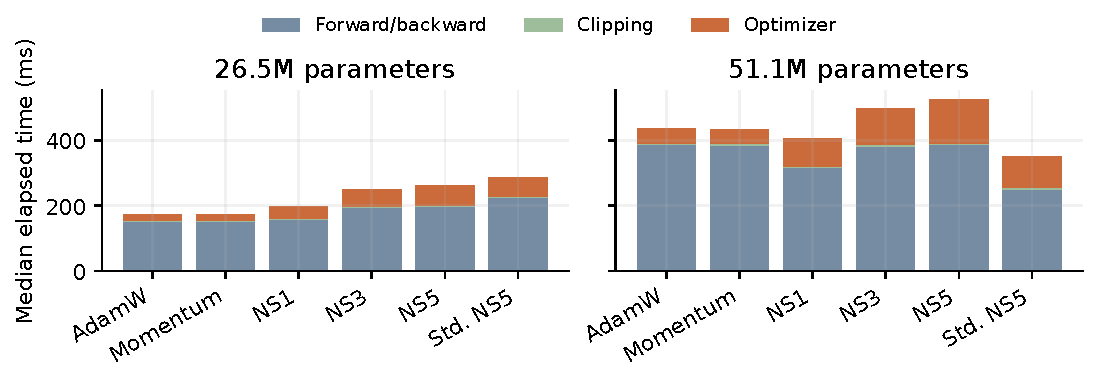
\includegraphics[width=\linewidth]{figures_v2/v2_profile.pdf}
\caption{同一模型规格下的同步计时。前向与反向、梯度裁剪和优化器分别取12次测量的中位数。}
\label{fig:v2profile}
\end{figure}
